\documentclass[11pt]{pk}
% \documentclass[en,11pt]{aghdpl}  % praca w języku angielskim

% Lista wszystkich języków stanowiących języki pozycji bibliograficznych użytych w pracy.
% (Zgodnie z zasadami tworzenia bibliografii każda pozycja powinna zostać utworzona zgodnie z zasadami języka, w którym dana publikacja została napisana.)
\usepackage[english,polish]{babel}

% Użyj polskiego łamania wyrazów (zamiast domyślnego angielskiego).
\usepackage{polski}

\usepackage[utf8]{inputenc}

% dodatkowe pakiety

\usepackage{mathtools}
\usepackage{amsfonts}
\usepackage{amsmath}
\usepackage{amsthm}

% --- < bibliografia > ---

\usepackage[
style=numeric,
sorting=none,
%
% Zastosuj styl wpisu bibliograficznego właściwy językowi publikacji.
language=autobib,
autolang=other,
% Zapisuj datę dostępu do strony WWW w formacie RRRR-MM-DD.
urldate=iso8601,
% Nie dodawaj numerów stron, na których występuje cytowanie.
backref=false,
% Podawaj ISBN.
isbn=true,
% Nie podawaj URL-i, o ile nie jest to konieczne.
url=false,
%
% Ustawienia związane z polskimi normami dla bibliografii.
maxbibnames=3,
% Jeżeli używamy BibTeXa:
backend=bibtex
]{biblatex}

\usepackage{csquotes}
% Ponieważ `csquotes` nie posiada polskiego stylu, można skorzystać z mocno zbliżonego stylu chorwackiego.
\DeclareQuoteAlias{croatian}{polish}

\addbibresource{bibliografia.bib}

% Nie wyświetlaj wybranych pól.
%\AtEveryBibitem{\clearfield{note}}


% ------------------------
% --- < listingi > ---

% Użyj czcionki kroju Courier.
%\usepackage{courier}

\usepackage{listings}
\lstloadlanguages{TeX}

\lstset{
	literate={ą}{{\k{a}}}1
           {ć}{{\'c}}1
           {ę}{{\k{e}}}1
           {ó}{{\'o}}1
           {ń}{{\'n}}1
           {ł}{{\l{}}}1
           {ś}{{\'s}}1
           {ź}{{\'z}}1
           {ż}{{\.z}}1
           {Ą}{{\k{A}}}1
           {Ć}{{\'C}}1
           {Ę}{{\k{E}}}1
           {Ó}{{\'O}}1
           {Ń}{{\'N}}1
           {Ł}{{\L{}}}1
           {Ś}{{\'S}}1
           {Ź}{{\'Z}}1
           {Ż}{{\.Z}}1,
	basicstyle=\footnotesize\ttfamily,
}

% ------------------------

\AtBeginDocument{
	\renewcommand{\tablename}{Tabela}
	\renewcommand{\figurename}{Rys.}
}

% ------------------------
% --- < tabele > ---

\usepackage{array}
\usepackage{tabularx}
\usepackage{multirow}
\usepackage{booktabs}
\usepackage{makecell}
\usepackage[flushleft]{threeparttable}

% defines the X column to use m (\parbox[c]) instead of p (`parbox[t]`)
\newcolumntype{C}[1]{>{\hsize=#1\hsize\centering\arraybackslash}X}


%---------------------------------------------------------------------------
\author{Łukasz Lalik}
\shortauthor{Ł. Lalik}

\titlePL{Interaktywna symulacja stosu protokołów LTE}
\titleEN{Interactive simulation of the LTE protocols stack}

\shorttitlePL{Interaktywna symulacja stosu protokołów LTE}
\shorttitleEN{Interactive simulation of the LTE protocols stack}

\thesistype{Praca magisterska}

\supervisor{dr inż. Jerzy Jaworowski}

\degreeprogramme{Teleinformatyka}

\date{2020}

\department{Katedra Teleinformatyki}
\faculty{Wdział Informatyki i Telekomunikacji}

\acknowledgements{Dla kogo?}
\nralbumu{D/130299}
\rodzajpracy{magisterska}
\miasto{Kraków}

\setlength{\cftsecnumwidth}{10mm}

%---------------------------------------------------------------------------
\setcounter{secnumdepth}{4}
\brokenpenalty=10000\relax

\begin{document}

\makepktitle

% Ponowne zdefiniowanie stylu `plain`, aby usunąć numer strony z pierwszej strony spisu treści i poszczególnych rozdziałów.
\fancypagestyle{plain}
{
	% Usuń nagłówek i stopkę
	\fancyhf{}
	% Usuń linie.
	\renewcommand{\headrulewidth}{0pt}
	\renewcommand{\footrulewidth}{0pt}
}

\setcounter{tocdepth}{2}
\tableofcontents
\clearpage

\chapter{Wprowadzenie}
\label{cha:wprowadzenie}

Od lat 80. XX wieku możemy zaobserwować coraz szybszy rozwój telefonii komórkowej. Osobom przyzwyczajonym do korzystania ze smartfona ze stałym dostępem do internetu w szybkiej sieci LTE lub 3G może wydawać się nieprawdopodobne, że kilkadziesiąt lat temu sieci pierwszej generacji (1G) pozwalały jedynie na rozmowy głosowe przesyłane analogowo (\cite{TanWet11}).

Sposób wykorzystania sieci komórkowej uległ znaczniej zmianie - zamiast transmisji, przede wszystkim połączeń głosowych, obecnie ruch sieciowy zdominowany jest przez transmisję danych w oparciu o protokół IP.

Infrastruktura sieci komórkowej musi wspierać coraz większą liczbę podłączonych urządzeń. Z kolei urządzenia wykorzystywane są już nie tylko do rozmów głosowych ale również do przesyłania wideo, muzyki, prowadzenia wideokonferencji oraz rozrywki elektronicznej. Dodatkowo użytkownicy oczekują, że dostęp do sieci będzie możliwy ciągle i w każdym miejscu bez zauważalnych spadków prędkości.


W odpowiedzi na to technologia dostępu zdalnego rozwija się w zawrotnym tempie co powoduje, że jest coraz bardziej złożona. Aby zrozumieć zasady jej działania obecnie potrzebne jest zdobycie rozległej wiedzy z zakresu przetwarzania sygnałów cyfrowych, sieci komputerowych, informatyki. Właśnie nad problemem wysokiego progu wejścia w technologię LTE postanowiłem się pokłonić w mojej pracy.

\section{Cele pracy}					
\label{sec:celePracy}

Celem pracy było przygotowanie interaktywnej symulacji stosu protokołów używanych w LTE po to, aby ułatwić jego zrozumienia osobie chcącej zapoznać się z tym systemem. Ilość mechanizmów obecnych LTE oraz ich wzajemnie zależności mogą stanowić wysoki próg wejścia dla osoby chcącej zagłębić się w ten system. Chociaż publicznie dostępna jest specjalistyczna literatura na ten temat to jednak często język w jakim jest pisana może nie być przystępny dla osób które dopiero poznają zagadnienia związane z zasadami działania LTE. 

\section{Zawartość pracy}
\label{sec:zawartoscPracy}

W mojej pracy skupiłem się na przygotowaniu symulacji oraz opisie podwarstw warstwy 2. stosu protokołów LTE. Ograniczyłem się również tylko do płaszczyzny danych użytkownika (user plane). Ostatecznie pozwoliło to symulować kompletny proces przesyłu pakietu IP od urządzenia użytkownika do stacji bazowej oraz od stacji bazowej do urządzenia użytkownika.

\begin{enumerate}%[1)]

\item Rozdział \ref{cha:protokoly} przedstawia ogólnie stos protokołów LTE
\item Rozdział \ref{cha:pdcp} skupia się na przedstawieniu zadań podwarstwy Packet Data Convergence Protocol
\item Rozdział \ref{cha:rlc} opisuje zakres odpowiedzialności podwarstwy Radio Link Control
\item W rozdziale \ref{cha:mac} opisano zadania podwarstwy Medium Access Control

\end{enumerate}

\chapter{Stos protokołów LTE}
\label{cha:protokoly}

Protokoły stosowane w systemach LTE możemy podzielić na 2 grupy: protokoły płaszczyzny użytkownika oraz protokoły płaszczyzny kontroli.

Protokoły płaszczyzny użytkownika (Rys. \ref{fig:userPlaneProtocols}) odpowiedzialne są za przesył danych użytkownika dostarczanych przez wyższe warstwy, np. przez warstwę Internet Protocol (IP). Natomiast protokoły płaszczyzny kontrolnej (Rys. \ref{fig:controlPlaneProtocols}) są odpowiedzialne za zarządzanie połączeniem poprzez konfigurację poszczególnych warstw płaszczyzny użytkownika lub zarządzanie zasobami radiowymi.

\begin{figure}
	\centering
		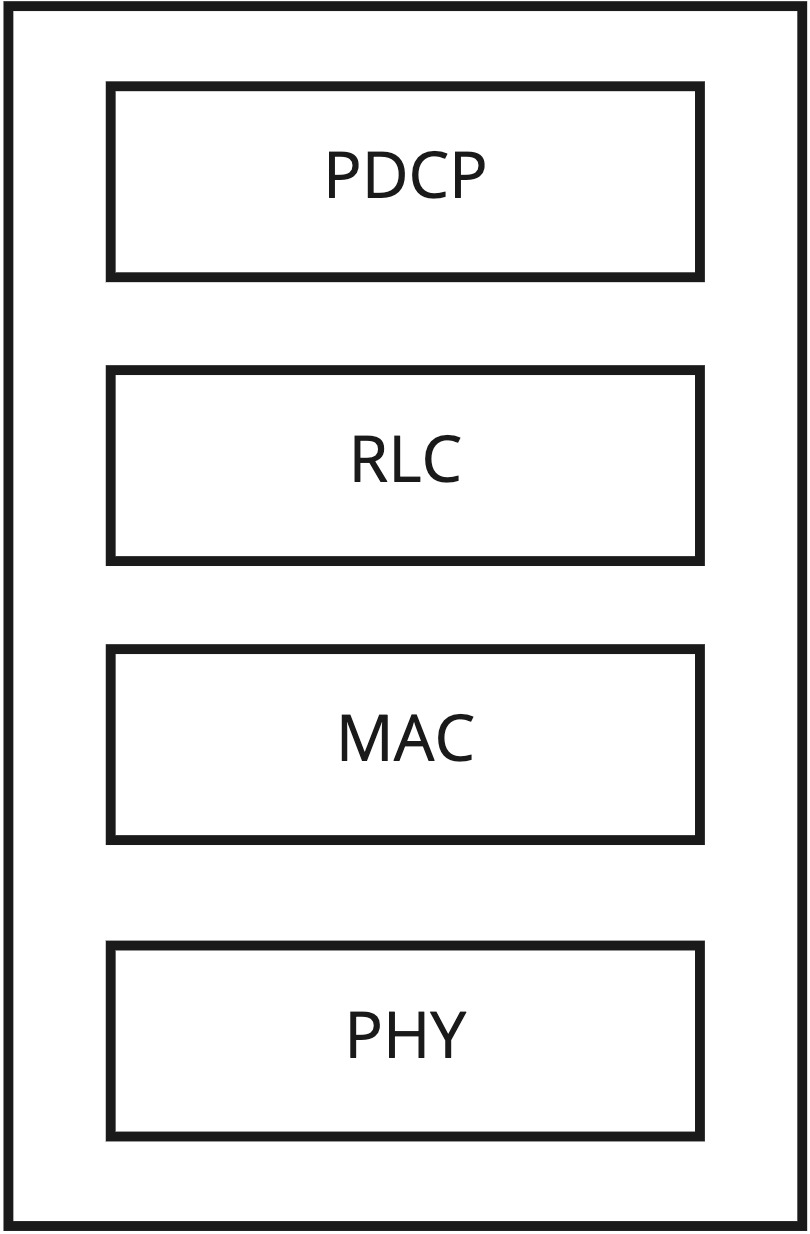
\includegraphics[width=0.2\textwidth]{user-plane-protocols.jpg}
	\caption{Stos protokołów dla płaszczyzny użytkownika}
	\label{fig:userPlaneProtocols}
\end{figure}


\begin{figure}
	\centering
		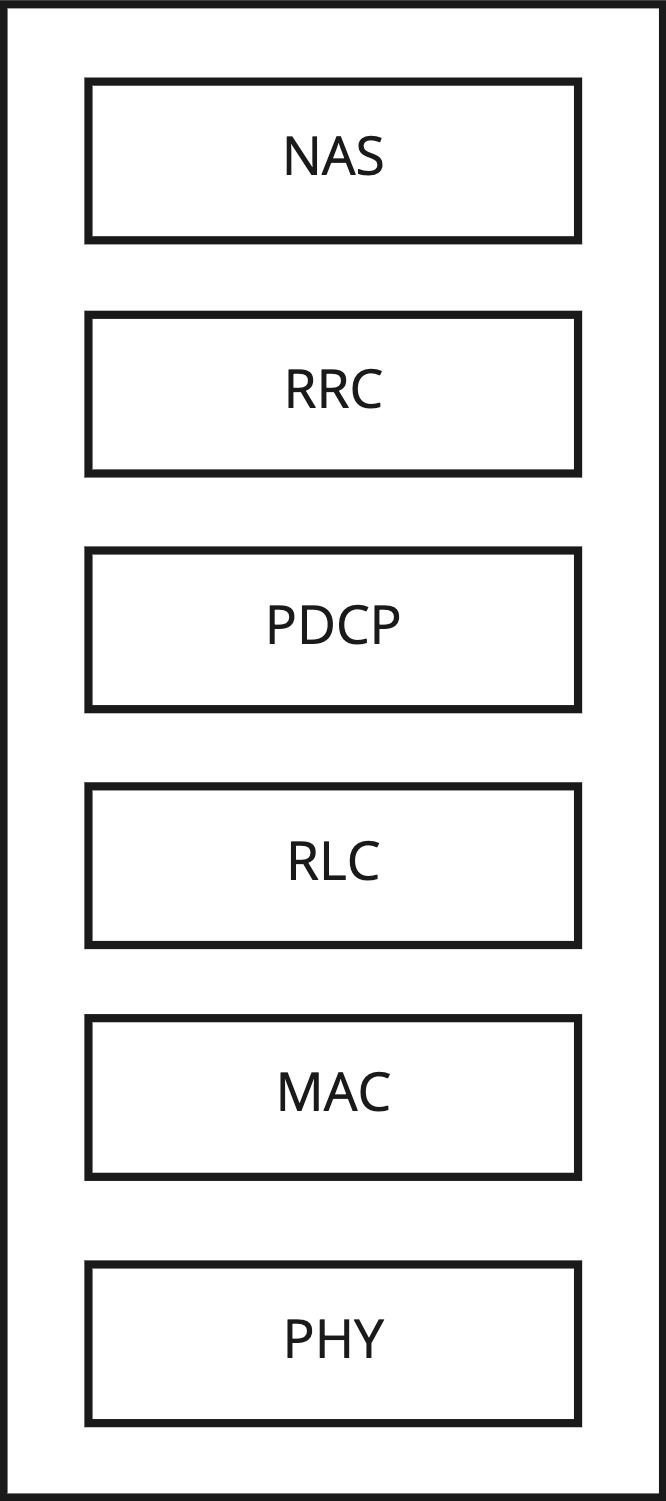
\includegraphics[width=0.2\textwidth]{control-plane-protocols.jpg}
	\caption{Stos protokołów dla płaszczyzny kontrolnej}
	\label{fig:controlPlaneProtocols}
\end{figure}


\chapter{Podwarstwa Packet Data Convergence Protocol}
\label{cha:pdcp}

\begin{figure}[ht]
	\centerline{\frame{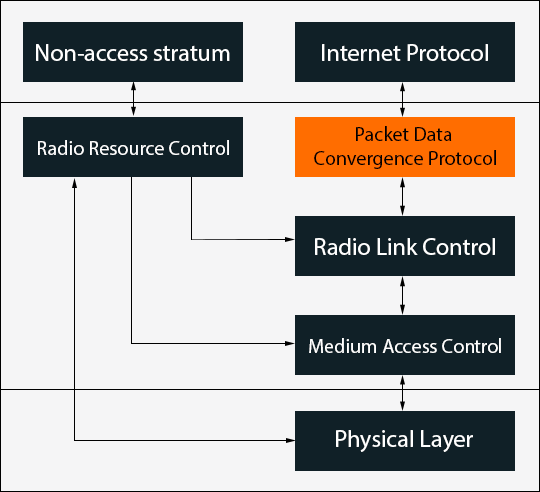
\includegraphics[width=0.5\textwidth]{images/pdcp_overview.png}}}
	\caption{Umiejscowienie podwarstwy PDCP w stosie protokołów LTE}
	\label{fig:pdcpseq}
\end{figure}

Podwarstwa PDCP (Packet Data Convergence Protocol) jest pierwszą z podwarstw z których składa się warstwa 2. stosu protokołów LTE. Dla każdego nośnika radiowego konfigurowana jest jej osobna instancja. Może ona odpowiadać za dane na płaszczyźnie użytkownika (wówczas świadczy usługi dla warstwy IP) lub za dane na płaszczyźnie kontroli i wówczas korzysta z niej warstwa RRC. Warstwa PDCP przesyła pakiety dalej do podwarstwy RLC.

W zależności od płaszczyzny danych, warstwa PDCP jest odpowiedzialna za:

Dla płaszczyzny kontroli:
\begin{enumerate}
	\item Dostarczenie danych w odpowiedniej kolejności i bez duplikatów
	\item Zapewnienie integralności danych
	\item Szyfrowanie danych
\end{enumerate}

Dla płaszczyzny danych użytkownika:
\begin{enumerate}
	\item Dostarczenie danych w odpowiedniej kolejności i bez duplikatów
	\item Kompresję nagłówków
	\item Szyfrowanie danych
\end{enumerate}

W projekcie skupiono się na symulacji przesyłu danych na płaszczyźnie danych użytkownika. Poniżej opisano proces przesyłu pakietu IP od urządzenia użytkownika (UE) do stacji bazowej (eNB) z perspektywy podwarstwy PDCP. Pomocniczo posłużono się zrzutami ekranu z wykonanej symulacji.

\section{Przetwarzanie pakietów IP na podwarstwie PDCP}

\subsection{Nadawanie numeru sekwencyjnego}

Pierwszym krokiem po otrzymaniu pakietu IP z warstwy sieciowej przez podwarstwę PDCP jest nadanie numeru sekwencyjnego. Pozwala on podwarstwie PDCP po stronie odbiornika odrzucić zduplikowane jednostki danych oraz dostarczyć je do wyższych warstw w odpowiedniej kolejności (Rys. \ref{fig:pdcpseq}). 
W tym celu po stronie nadajnika utrzymywany jest liczniki, którego aktualna wartość jest przypisywana jako numer sekwencyjny nowo otrzymanemu pakietowi a następnie inkrementowana. Z kolei po stronie odbiornika odebrane pakiety są umieszczane w buforze gdzie następnie są sortowane na podstawie numeru sekwencyjnego i przekazywane w odpowiedniej kolejności do wyższych warstw.

\begin{figure}[ht]
	\centerline{\frame{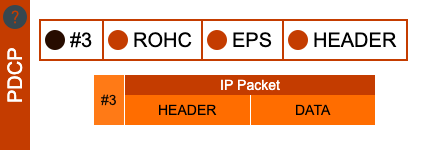
\includegraphics[width=0.5\textwidth]{images/pdcp_1.png}}}
	\caption{Nadanie numeru sekwencyjnego pakietowi IP}
	\label{fig:pdcpseq}
\end{figure}

\subsection{Kompresja metodą ROHC (Robust Header Compression)}

Drugim krokiem jest kompresja nagłówka pakietu IP przy użyciu metody ROHC (Robust Header Compression). Ogólna zasada działania opiera się na założeniu, że jeżeli pakiety IP wysyłane są pomiędzy dwoma urządzeniami wówczas większość pól w ich nagłówkach jest taka sama. W przypadku pakietu IPv4 rozmiar nagłówka wynosi 20 bajtów. Jeżeli jest on użyty w połączeniu z protokołami UDP i RTP wówczas rozmiar nagłówka w sumie wynosi 40 bajtów. ROHC pozwala zmniejszyć rozmiar takiego nagłówka do 2 - 4 bajtów. Warto również zauważyć, że protokół RTP używany zazwyczaj w kodowaniu głosu w czasie rzeczywistym transportuje niewielkie ilości danych w pojedynczym pakiecie - zazwyczaj 20 - 40 bajtów. Porównując to z nieskompresowanym nagłówkiem o ilości 40 bajtów widać, że narzut nagłówka jest znaczny. Dzięki temu zastosowanie kompresji ROHC pozwala zaoszczędzić znaczną część pasma.

\subsection{Szyfrowanie}

Po kompresji następuje szyfrowanie danych zawartych w pakiecie. Zarówno algorytm jak i klucz użyty do szyfrowania jest konfigurowany przez wyższe warstwy. Podczas konstruowania klucza szyfrującego używane są parametry takie jak COUNT (kombinacja numeru sekwencyjnego i numeru ), DIRECTION (kierunek transmisji) oraz parametry dostarczane przez wyższe warstwy, takie jak BEARER (5-bitowy identyfikator nośnika radiowego) oraz KEY (128-bitowy klucz szyfrujący).

\begin{figure}[ht]
	\centerline{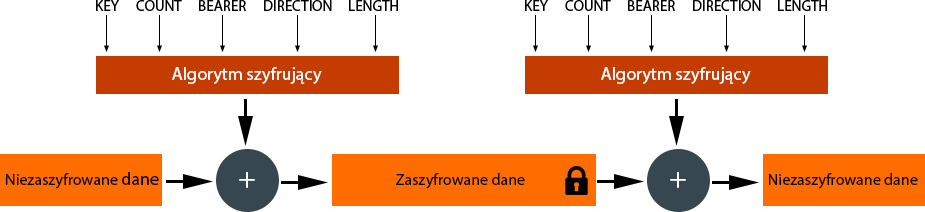
\includegraphics[width=0.9\textwidth]{images/pdcp-eps.png}}
	\caption{Wizualizacja metody szyfrowania danych}
\end{figure}

\subsection{Format wyjściowej jednostki danych (PDU) dla podwarstwy PDCP}

Ostatnim krokiem jest dodanie nagłówków warstwy PDCP i zbudowanie pakietu PDU dla warstwy PDCP. Nagłówek składa się z:
\begin{itemize}
	\item 1-bitowej informacji o tym czy pakiet zawiera dane płaszczyzny użytkownika czy dane płaszczyzny kontroli wygenerowane przez podwarstwę PDCP (pole D/C na rysunkach \ref{fig:pdcp7bit} i \ref{fig:pdcp12bit})
	\item numeru sekwencyjnego zapisanego przy użyciu 7 lub 12 bitów
	\item w przypadku 12-bitowego numeru sekwencyjnego, jest on poprzedzony trzema nieużywanymi bitami zarezerwowanymi do ewentualnego użycia w przyszłości (pola R na rysunku \ref{fig:pdcp12bit})
\end{itemize}

\begin{figure}[ht]
	\centerline{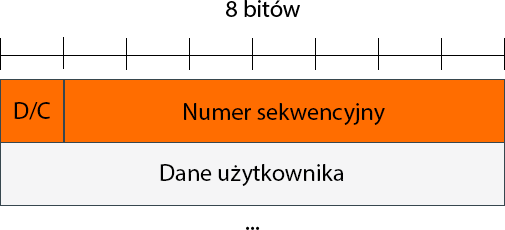
\includegraphics[width=0.4\textwidth]{images/pdcp-pdu-7bit.png}}
	\caption{Pakiet PDU dla warstwy PDCP z 7-bitowym numerem sekwencyjnym}
	\label{fig:pdcp7bit}
\end{figure}

\begin{figure}[ht]
	\centerline{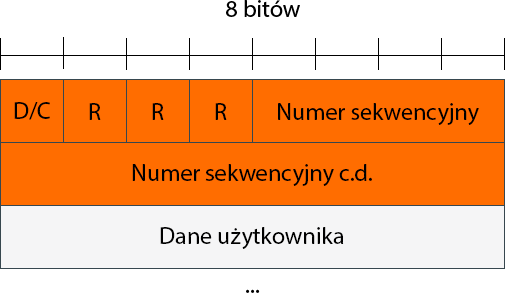
\includegraphics[width=0.4\textwidth]{images/pdcp-pdu-12bit.png}}
	\caption{Pakiet PDU dla warstwy PDCP z 12-bitowym numerem sekwencyjnym}
	\label{fig:pdcp12bit}
\end{figure}
\chapter{Podwarstwa Radio Link Control}
\label{cha:rlc}

\begin{figure}
	\centerline{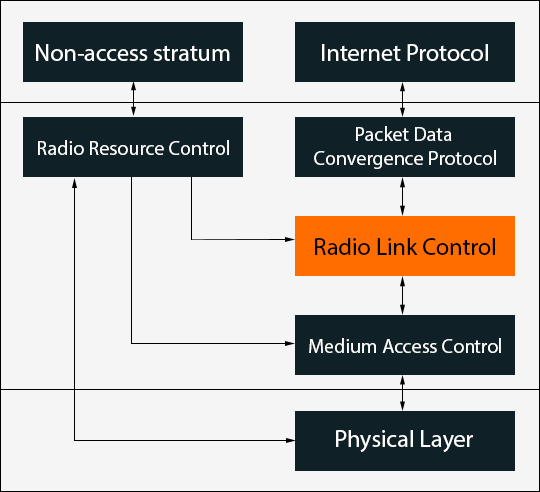
\includegraphics[width=0.4\textwidth]{images/rlc_overview.png}}
	\caption{Umiejscowienie podwarstwy RLC w stosie protokołów LTE}
	\label{fig:rlc_overview}
\end{figure}

Podwarstwa RLC (Radio Link Control) jest drugą z podwarstw warstwy 2. Odbiera ona jednostki danych z podwarstw PDCP oraz RRC a następnie przekazuje je do podwarstwy MAC. RLC może działać w jednym z 3 trybów transmisji: transparentnym, z potwierdzeniami lub bez potwierdzeń. Jest ona odpowiedzialna za:

\begin{enumerate}
	\item Segmentację i/lub łączenie transmitowanych jednostek danych
	\item Wykrywanie zduplikowanych jednostek danych podczas ich odbierania z niższych warstw
	\item Zapewnienie dostarczenia jednostek danych w odpowiedniej kolejności
	\item Naprawa błędów poprzez ponowne wysyłanie jednostek danych
\end{enumerate}

\section{Segmentacja i łączenie jednostek danych}
\label{sec:segmentation}

Zanim podwarstwa RLC po stronie urządzenia transmitującego prześle dane do odbiornika musi poczekać na informację z podwarstwy MAC o tym, że własnie pojawiła się możliwość transmisji danych. Do tego czasu podwarstwa RLC przechowuje jednostki danych, które otrzymała z wyższych warstw w buforze transmisyjnym (Transmission Buffer na Rys. \ref{fig:rlc_simulation}). Razem z informacją o możliwości transmisji podwarstwa MAC wysyła również informację o rozmiarze bloku transportowego czyli o tym jaka ilość danych może zostać przesłana. Rozmiar dostępnego bloku transportowego może być za każdym razem inny i zależy on m.in. od jakości połączenia. Z tego powodu podwarstwa RLC musi dostosowywać rozmiar jednostek danych wysyłanych do podwarstwy MAC do rozmiaru bloku transportowego. \cite{Perez15}

W tym celu jednostki danych, zbyt duże aby w całości zmieścić się w bloku transportowym, są dzielone na mniejsze fragmenty i wysyłane w dwóch lub więcej blokach transportowych. Natomiast jeżeli jednostki danych są dużo mniejsze od bloku transportowego to kilka jednostek danych jest umieszczonych w pojedynczym bloku transportowym. Dzięki temu dostępna przepustowość jest wykorzystywana maksymalnie efektywnie. Po stronie odbiornika odebrane jednostki danych są umieszczane w buforze. Jeżeli możliwe jest z nich odtworzenie kompletnej jednostki danych wówczas są one łączone i wysyłane do wyższej warstwy.

Na Rys. \ref{fig:rlc_simulation} przedstawiono zrzut ekranu z wykonanej symulacji przedstawiający podwarstwę RLC. W centralnej części widoczny jest blok transportowy zawierający 3 jednostki SDU, które były na tyle małe aby razem, w całości zmieścić się w bloku transportowym.

\begin{figure}
	\centerline{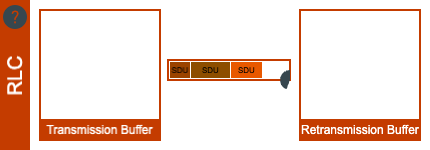
\includegraphics[width=0.5\textwidth]{images/rlc_transport_block.png}}
	\caption{Segmentacja SDU w bloku transportowym}
	\label{fig:rlc_simulation}
\end{figure}
  
\section{Wykrywanie zduplikowanych jednostek danych}

Błędy podczas transmisji danych mogą spowodować, że niektóre jednostki danych dotrą do odbiornika więcej niż raz. Warstwa RLC odpowiada za wykrycie zduplikowanych pakietów a następnie odrzucenie ich tak aby nie zostały ona przekazane do wyższych warstw. W tym celu każda jednostka danych podczas wysyłania posiada w nagłówku przypisany numer sekwencyjny. Z kolei odbiornik po swojej stronie utrzymuje bufor z odebranymi jednostkami danych. Jeżeli nowo odebrana jednostka danych posiada taki sam numer sekwencyjny jak jednostka danych która znajduje się w buforze oznacza to, że jest ona duplikatem i zostaje odrzucona.

\section{Zapewnienie kolejności}

Numer sekwencyjny, przypiswany do jednostek danych, jest również wykorzystywany do zapewnienia aby jednostki danych po stronie odbiornika były dostarczone przez podwarstwę RLC do wyższych warstw w tej samej kolejności w jakiej zostały one wysłane po stronie nadajnika. Oznacza to, że jednostka danych o numerze sekwencyjnym N musi zostać dostarczona przed jednostką danych o numerze sekwencyjnym N+1. Mechanizm ten działa w odmienny sposób dla trybu transmisji z potwierdzeniami i bez potwierdzeń dlatego też został dokładniej opisany w sekcjach \ref{subsec:um} i \ref{subsec:am}.

\section{Korekcja błędów}

O ile usługi typu VoIP mogą działać prawidłowo nawet jeżeli niewielka liczba pakietów nie dotrze od nadajnika do odbiornika to usługi typu HTTP lub FTP nie będa dziąłać prawidłowo jeżeli jakiekolwiek dane zostaną utracone. W tym celu podwarstwa RLC implementuje mechanizm ARQ (Automatic Repeat Request) który ma za zadanie wykrycie czy jakieś jednostki danych nie zostały dostarczone i zarządanie od nadawacy aby ponowił ich wysłanie. Mechanizm ten jest używany tylko w trybie transmisji z potwierdzeniami.

Po stronie odbiornika każda otrzymana jednostka danych jest weryfikowana pod kątem poprawności. W tym celu najczęściej używany jest mechanizm CRC (Cyclic Redundancy Check). Jeżeli odbiorca stwierdzi, że otrzymana jednostka danych jest błędna wysyła żądanie jej ponownej transmisji (NACK). Natomiast jednostka danych zostanie uznana za prawidłową zostaje wysłane potwierdzenie poprawnej transmisji (ACK). Po stronie nadawcy również dla każdej wysłanej jednostki danych startowany jest zegar, który odlicza czas do ponownej transmisji tej jednostki. Jeżeli przed upływem tego czasu zostanie otrzymane potwierdzenie (ACK) zegar jest zatrzymywana i jednostka danych usuwana z bufora po stronie nadawcy. W przeciwnym wypadku po upływie czasu jednostka danych jest ponownie transmitowana i odliczanie ponowione. Cały proces powtarza się dopóki nie zostanie odebrane potwierdzenie od odbiorcy lub dopóki cała komunikacja nie zostanie anulowana.


Wyróżnia się trzy typy mechanizmu ARQ:

\begin{enumerate}
	\item Stop-and-Wait ARQ - jest to najbardziej podstawowa forma mechanizmu ARQ. Nadawca wysyła jeden pakiet i oczekuje na potwierdzenie (ACK) lub żadanie ponownej transmisji (NACK) od odbiorcy a także startuje licznik czasowy. Jeżeli przed upływem czasu nie otrzyma potwierdzenia lub jeżeli otrzyma żadanie ponownej transmisji wówczas ponownie wysyła ten sam pakiet. Dopiero kiedy otrzyma od odbiorcy potwierdzenie (ACK) wówczas wysyła kolejny pakiet.
	\item Go-Back-N ARQ - w tym trybie określony jest pewien rozmiar okna transmisyjnego - N. Nadawca wysyła do N pakietów do odbiorcy a następnie oczekuje na ich potwierdzenia (ACK). Następnie sprawdza, które pakiety zostały potwierdzone i wznawia wysyłanie od pakietu o numerze sekwencyjnym, który jest kolejny po ostatnio potwierdzonym pakiecie. Odbiorca utrzymuje po swojej stronie informację o numerze sekwencyjnym następnego pakietu, który powinien dostać i ignoruje otrzymane pakiety jeżeli nie mają dokładnie tego numeru sekwencyjnego. Kiedy już otrzyma pakiet o wymaganym numerze sekwencyjnym wówczas wysyła do nadawcy potwierdzenie otrzymania pakietu (ACK) z załączonym numerem sekwencyjnym a następnie zwiększa u siebie oczekiwany numer sekwencyjny następnego pakietu o 1.
	\item Selective Repeat ARQ - w tym trybie również używane jest okno transmisyjne o danym rozmiarze - N. Nadawca wysyła N pakietów od odbiorcy. Odbiorca akceptuje kolejne pakiety, nawet jeżeli, któryś wcześniejszy pakiet był błędny lub nie dotarł. Odbiorca utrzymuje po swojej stronie najmniejszy numer sekwencyjny pakietu, który nie dotarł (lub był błędny) i wysyła go z każdym potwierdzeniem odebrania pakietów. Nadawca po wysłaniu N pakietów ponawia wysłanie pakietów, które nie dotarły do odbiorcy a następnie kontynuje wysyłanie pakietów od miejsca gdzie skończył.
\end{enumerate}

\section{Tryby transmisji}

\subsection{Transparentny}

Transparentny tryb transmisji jest używany przy przesyłaniu danych do kanałów sygnałowych takich jak BCCH, PCCH i CCCH. W tym trybie transmisji jednostki danych są przekazywane z wyższych warstw do niższych w niezmienionej postaci. Nie są dodawane żadne nagłówki więc jednostka danych wysyłana do niższych warstw jest taka sama jak jednostka danych otrzymana z warstwy wyższej (Rys. \ref{fig:rlc_tm_pdu}). Większość mechanizmów RLC nie jest używana. Jedynym wykorzystywanym mechanizmem jest bufor transmisyjny w którym jednostki danych są przechowywane dopóki podwarstwa MAC nie poinformuje o możliwości transmisji danych.

\begin{figure}
	\centerline{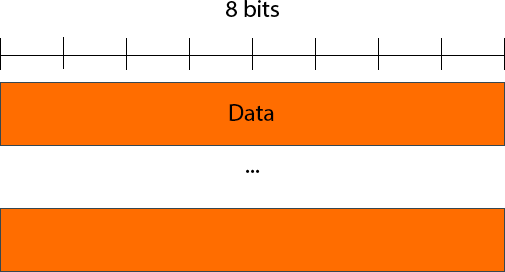
\includegraphics[width=0.3\textwidth]{images/rlc_tm_pdu.png}}
	\caption{Struktura pakietu PDU dla transparentnego trybu transmisji}
	\label{fig:rlc_tm_pdu}
\end{figure}

\subsection{Bez potwierdzeń}
\label{subsec:um}

W trybie transmisji bez potwierdzeń dane przesyłane są poprzez kanał DTCH. Ten tryb jest używany przy serwisach gdzie utrata niewielkiej ilości pakietów jest akceptowalna (np. serwis VoIP). W pierwszej kolejności podlegają one procesowi segmentacji i/lub łączenia. Następnie dodawany jest nagłówek specyficzny dla transmisji bez potwierdzeń (Rys. \ref{fig:rlc_um_pdu}) zawierający: 

\begin{figure}
	\centerline{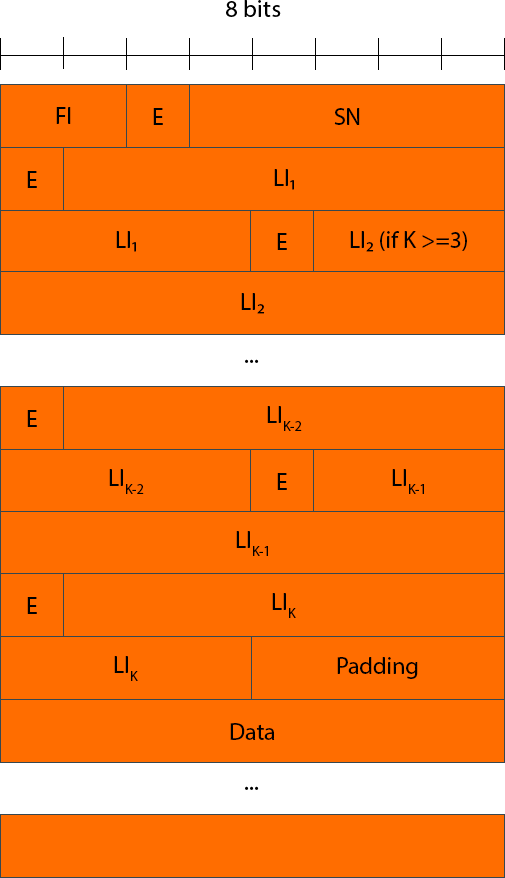
\includegraphics[width=0.3\textwidth]{images/rlc_um_pdu.png}}
	\caption{Struktura pakietu PDU dla trybu transmisji bez potwierdzeń}
	\label{fig:rlc_um_pdu}
\end{figure}

\begin{enumerate}
	\item FI (2 bity) informuje czy na poczatku i/lub na końcu pakietu znajdują się posegmentowane jednostki danych	
	\item E (1 bit) informuje czy dalsza część pakietu zawiera pola LI
	\item SN (10 bitów) numer sekwencyjny pakietu
	\item LI (11 bitów) zawiera informację jaki rozmiar ma transportowana jednostka danych. Jeżeli w pakiecie transportowane jest więcej jednostek danych to tyle samo razy w nagłówku pojawia się pole E i LI
\end{enumerate}

 Jeżeli podwartwa RLC po stronie odbiornika otrzyma zduplikowaną jednostkę danych to zostaje ona odrzucona. Jeżeli jednostka danych dotrze w złej kolejności, lub jeżeli jakaś jednostka danych nie dotrze w ogóle wówczas jest to ignorowane i wykorzystywane są tylko te jednostki danych, które dotarły w prawidłowej kolejności. Do wyższych warstw dostarczane są tylko te jednostki danych, które udało się w całości odtworzyć. 

\subsection{Z potwierdzeniami}
\label{subsec:am}

Tryb transmisji z potwierdzeniami jest najbardziej złożony i to właśnie na nim skupiono się w przygotowanej symulacji. Jest on używany w serwisach w których do ich prawidłowego działania konieczne jest dostarczenie pakietów bez błędów, bez duplikatów i w odpowiedniej kolejności. W transmisji z potwierdzeniami wykorzystywane są kanały DCCH oraz DTCH. W pierwszej kolejności jednostki danych podlegają procesowi segmentacji i/lub łączenia tak aby zmieścić się i maksymalnie wykorzystać przestrzeń dostępną w bloku transportowym zdeklarowanym przez podwarstwę MAC. Wysłane jednostki danych następnie trafiają do bufora retransmisji. Jeżeli odbiorca potwierdzi odebrane jednostki danych zostaje ona usunięta z bufora retransmisji. Jeżeli jednak odbiorca wyśle zapytanie o ponowną transmisję jednostki danych wówczas zostanie ona pobrana z bufora retransisji i wysyłana ponownie. Należy zauważyć, że podczas ponownej transmisji dostępny blok transportowy może mieć już inny rozmiar. W tym celu jednostki danych z bufora rentransmisji mogą wymagać ponownej segmentacji i/lub łączeniu aby dostosować ich rozmiar do nowego bloku transportowego.

Na Rys. \ref{fig:rlc_am_pdu} przedstawiono strukturę pakietu PDU dla transmisji z potwierdzeniami. Składa się on z następujących elementów:

\begin{enumerate}
	\item D/C (1 bit) informuje czy pakiet jest przeznaczony dla User Plane czy dla Control Plane
	\item RF (1 bit) informuje czy pakiet zawiera posegmentowaną jednostkę danych, która jest ponownie wysyłana
	\item P (1 bit) polling Bit informuje czy odbiorca powinien wysłać do nadawcy pakiet status PDU
	\item FI (2 bity) informuje czy na poczatku i/lub na końcu pakietu znajdują się posegmentowane jednostki danych
	\item E (1 bit) informuje czy dalsza część pakietu zawiera pola LI
	\item SN (10 bitów) numer sekwencyjny pakietu
	\item LI (11 bitów) zawiera informację jaki rozmiar ma transportowana jednostka danych. Jeżeli w pakiecie transportowane jest więcej jednostek danych to tyle samo razy w nagłówku pojawia się pole E i LI
\end{enumerate}

\begin{figure}
	\centerline{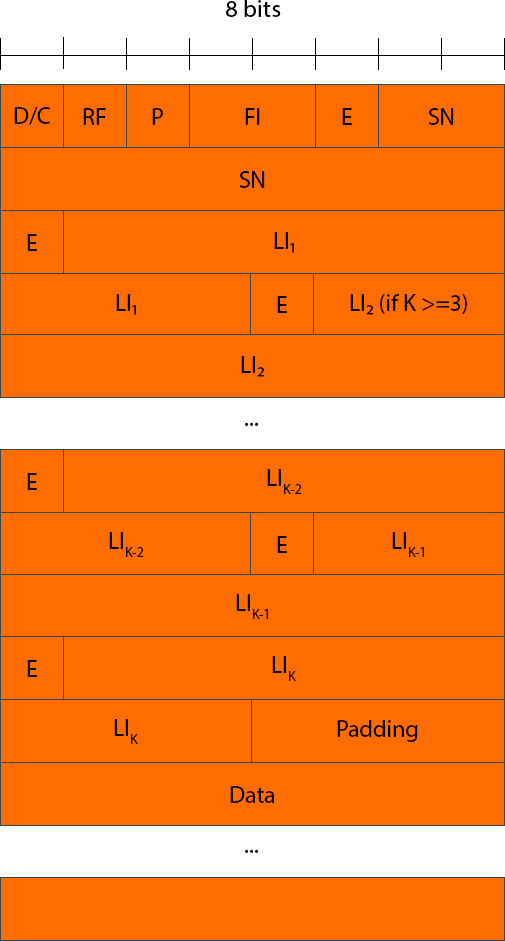
\includegraphics[width=0.3\textwidth]{images/rlc_am_pdu.png}}
	\caption{Struktura pakietu PDU dla transmisji z potwierdzeniami}
	\label{fig:rlc_am_pdu}
\end{figure}

Po stronie odbiornika w pierwszej kolejności następuje odrzucenie zduplikowanych jednostek danych jezeli takie zostaną wykryte. Następnie jednostki danych zostają umieszczone w buforze danych gdzie zostają zorganizowane w odpowiedniej kolejności (wg numeru sekwencyjnego). Zostają one wysłane do wyższych warstw dopiero wtedy gdy możliwe jest odtworzenie z nich kompletnej jednostki danych i nie ma wcześniejszych brakujących jednostek danych. Jeżeli któreś jednostki danych nie dotarły lub zawierają błędy wówczas wysyłane jest żądanie (NACK) do nadajnika o ponowną transmisję brakujących jednostek danych. Dla jednostek danych, które dotarły bez błędów i w prawidłowej kolejności wysyłane jest potwierdzenie dostarczenia (ACK).

Żądnie ponownego wysłania pakietu jak i potwierdzenie dostarczenia pakietu zawarte jest w jednostce danych nazywanej Status PDU przedstawionej na Rys. \ref{fig:status_pdu}. Składa się ona z następujących elementów:

\begin{enumerate}
	\item D/C (1 bit) informuje czy pakiet jest przeznaczony dla User Plane czy dla Control Plane
	\item CPT (3 bity) zawiera informację o typie pakietu przeznaczonego dla Control Plane
	\item ACK SN (10 bitów) zawiera numer sekwencyjny o 1 większy od numeru sekwencyjnego ostatnio poprawnie odebranego pakietu
	\item NACK SN (10 bitów) zawiera numer sekwencyney pakietu uznanego za utracony po stronie odbiornika
	\item E1 (1 bit) informuje czy dalsza część pakietu zawiera pola NACK SN, E1 i E2
	\item E2 (1 bit) informuje czy po polu NACK SN znajdują się pola SO start i SO end
	\item SO start (15 bitów) i SO end (15 bitów) wskazują na pozycję pierwsze i ostatniego bajtu jednostki danych która nie została prawidłowo odebrana
\end{enumerate}

\begin{figure}
	\centerline{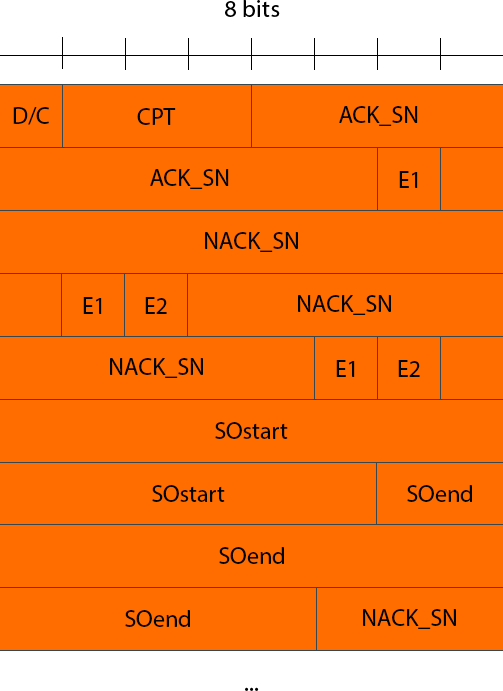
\includegraphics[width=0.3\textwidth]{images/rlc_status_pdu.png}}
	\caption{Struktura pakietu Status PDU}
	\label{fig:status_pdu}
\end{figure}

Aby została ona wysłana musi zajść jedna z dwóch sytuacji:
\begin{enumerate}
	\item Licznik czasowy T status prohibit zakonczył odliczanie i została odebrana jednostka danych z włączoną flagą poll bit
	\item Liczniki czasowe T status prohibit i T reordering zakończyły odliczanie
\end{enumerate}

Licznik czasowy T status prohibit zapewnia, że ten sam pakiet status PDU nie zostanie wysłany kilkakrotnie. Jego odliczanie jest wznawiane po każdym wysłaniu pakietu status PDU.

Licznik czasowy T reordering jest startowany wówczas, gdy zostaną zauważone brakujące pakiety tj. gdy zostanie odebrany pakiet o numerze sekwencyjnym N a nie został jeszcze odebrany pakiet o numerze sekwencyjnym N - 1.

Flaga poll bit jest ustawiana po stronie nadajnika w następujących sytuacjach:
\begin{enumerate}
	\item Jeżeli pakietów wysłanych od czasu ostatniego potwierdzenia przekroczyła liczbę określoną przez parametr Poll PDU
	\item Jeżeli liczba bajtów wysłanych do odbiornika od czasu ostatniego potwierdzenia przekroczyła liczbę określoną przez parametr Poll Byte
	\item Jeżeli licznik czasowy T poll retransmit zakończył odliczanie i nie ma żadnych pakietów w buforze transmisji lub retransmisji (wówczas ponownie wysyłany jest ostatnio wysłany pakiet danych z ustawioną flagą poll bit)
\end{enumerate}
\chapter{Podwarstwa Medium Access Control}
\label{cha:mac}

Podwarstwa MAC (Medium Access Control) jest trzecią z podwarstw warstwy 2. Z podwarstwą RLC komunikuje się ona za pośrednictwem kanałów logicznych (logical channels) i wymienia z nią jednostki danych (SDU). Natomiast z warstwą fizyczną (PHY) komunikuje się przy użyciu kanałów transportowych (transport channels) i odbiera oraz przekazuje do niej dane w formie bloków transportowych. \cite{Cox14}

\begin{figure}
	\centerline{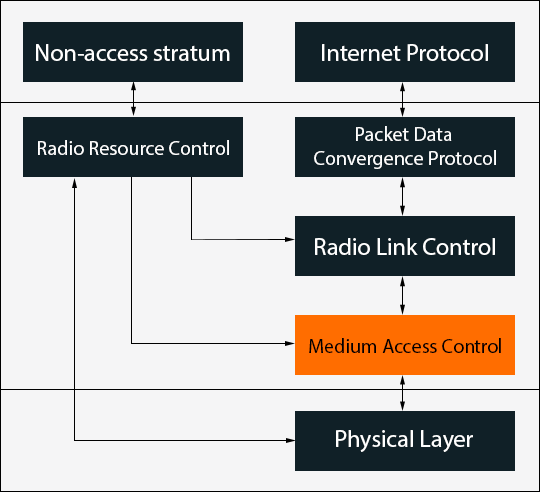
\includegraphics[width=0.4\textwidth]{images/mac_overview.png}}
	\caption{Umiejscowienie podwarstwy MAC w stosie protokołów LTE}
	\label{fig:mac_overview}
\end{figure}

Do funkcji podwarstwy MAC możemy zaliczyć:

\begin{enumerate} 
	\item Mapowanie jednostek danych (SDU) przesyłanych do kanałów logicznych na kanały transportowe, gdzie formowane są w bloki transportowe zawierające PDU
	\item Planowanie jak i kiedy jednostki danych mają zostać dostarczone
	\item Swobodny dostęp
	\item Zarządzenie synchronizacją czasu pomiędzy urządzeniem użytkownika a stacją bazową 
\end{enumerate}

\section{Mapowanie kanałów}

Podwarstwa MAC komunikuje się z podwarstwą RLC za pośrednictwem kanałów logicznych. Można je podzielić na kanały ``control channels`` transportujące dane dotyczące ``control plane`` oraz na kanały ''traffic channels'' transportujące dane dotyczące ''control plane''.

Wyróżniamy następujące kanały logiczne typu ``control channels``:

\begin{enumerate}
	\item Broadcast Control Channel (BCCH) - służy do publikowania informacji systemowych przeznaczonych do wszystkich urządzeń użytkownika w zasięgu danej stacji bazowej
	\item Paging Control Channel (PCCH) - służy do informowania urządzeń użytkownika o zdarzeniach zachodzących w sieci
	\item Common Control Channel (CCCH) - pozwala na przesyłanie informacji kontrolnych w dwóch kierunkach pomiędzy urządzeniem użytkownika i stacją bazową (dotyczy urządzeń, które nie ustanowiły połączenia na poziomie warstwy RRC)
	\item Multicast Control Channel (MCCH) - służy do publikowania informacji kontrolnych od stacji bazowej do wielu urządzeń użytkownika w ramach tzw. Multimedia Broadcast Multicast Services (MBMS)
	\item Dedicated Control Channel (DCCH) - pozwala na przesyłanie informacji kontrolnych w dwóch kierunkach pomiędzy urządzeniem użytkownika i stacją bazową (dotyczy urządzeń, które ustanowiły połączenie na poziomie warstwy RRC)
\end{enumerate}

Kanały logiczne typu ``traffic channels`` są następujące:

\begin{enumerate}
	\item Dedicated Traffic Channel (DTCH) - kanał przeznaczony do transportu danych użytkownika w dwóch kierunkach pomiędzy urządzeniem użytkownika oraz stacją bazową
	\item Multicast Traffic Channel (MTCH) - służy do publikowania danych od stacji bazowej do wielu urządzeń użytkownika w ramach MBMS
\end{enumerate}

Z warstwą fizyczną (PHY), podwarstwa MAC komunikuje się przy użyciu kanałów transportowych ``transport channels``. Dzielimy na kanały, które wysyłają dane od stacji bazowej do urządzenia użytkownika tzw. ``downlink channels`` oraz kanały używane do wysyłania danych od urządzenia użytkownika do stacji bazowej ``uplink channels``.

Wyróżniamy następujące ``downlink channels``:

\begin{enumerate}
	\item Broadcast Channel (BCH) - ten kanał posiada jeden predefiniowany format przesyłania danych a także przesyła dane do wszystkich urządzeń w zasięgu danej stacji bazowej
	\item Downlink Shared Channel (DL-SCH) - wspiera korekcję błędów HARQ, dostosowywanie formatu przesyłania danych, umożliwia przesyłanie danych zarówno do pojedynczego urządzenia jak i do wielu urządzeń równocześnie, posiada wsparcie dla UE DRX w celu oszczędzania energii
	\item Paging Channel (PCH) - przesyła dane do wszystkich urządzeń w zasięgu danej stacji bazowej. Posiada wsparcia dla UE DRX, 
	\item Multicast Channel (MCH) - publikuje dane do wszystkich urządzeń w zasięgu stacji bazowej
\end{enumerate}

Oraz następujące ``uplink channels``:

\begin{enumerate}
	\item Uplink Shared Channel (UL-SCH) - oferuje wsparcie dla korekcji błędów HARQ, oferuje dynamiczne dostosowywanie parametrów połączenia 
	\item Random Access Channel (RACH)
\end{enumerate}

\begin{figure}
	\centerline{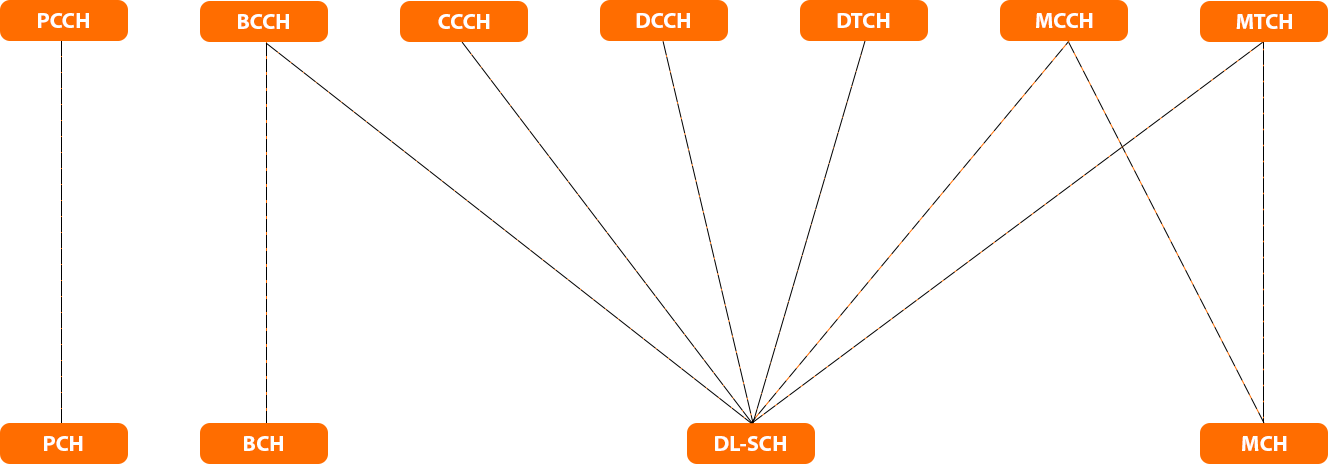
\includegraphics[width=0.8\textwidth]{images/mac_downlink_mapping.png}}
	\caption{\mbox{Mapowanie kanałów logicznych na transportowe dla downlink channels}}
	\label{fig:mac_downlink_mapping}
\end{figure}

\begin{figure}
	\centerline{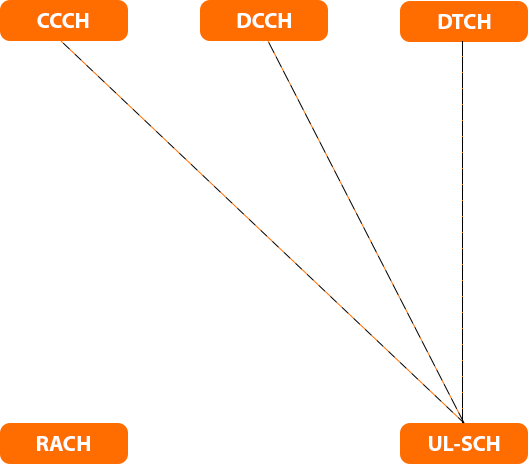
\includegraphics[width=0.5\textwidth]{images/mac_uplink_mapping.png}}
	\caption{Mapowanie kanałów logicznych na transportowe dla uplink channels}
	\label{fig:mac_uplink_mapping}
\end{figure}

\section{Elementy kontrolne podwarstwy MAC}
\label{sec:mac_control_elements}

Oprócz transmisji danych użytkownika podwarstwa MAC odpowiada za wysyłanie oraz odbieranie tzw. elementów kontrolnych (MAC control elements). Wpływają one na zachowanie warstwy fizycznej. Elementy kontrolne wymieniono oraz opisano w Tabeli \ref{tab:mac_control_elements}

\begin{center}
\begin{table}
	\begin{tabular}{ | m{8em} | m{30em} | }
		\hline
		Element kontrolny & Odpowiedzialność \\
		\hline
		Buffer status report & Informacja o stanie bufora danych po stronie urządzenia użytkownika \\
		\hline
		C-RNTI & Identyfikacja urządzenia użytkownika podczas swobodnego dostępu \\
		\hline
		Power headroom & Informacja o dostępnej mocy transmisyjnej urządzenia użytkownika \\
		\hline
		Extended power headroom & Dostępna moc transmisyjna podczas łączenia nośników danych \\
		\hline
		DRX command & Przełącza urządzenie użytkownika w tryb uśpienia \\
		\hline
		Timing advance command & Dostosowuje postęp czasowy w urządzeniu użytkownika \\
		\hline
		UE contention resolution identity & Rozwiązuje problem z rywalizacją o dostęp do kanału transmisyjnego pomiędzy urządzeniami użytkownika podczas swobodnego dostępu \\
		\hline
		MCH scheduling information & Przesyła informacje do urządzenia użytkownika związane z planowaniem MBMS \\
		\hline
		Activation / deactivation & Aktywuje / deaktywuje dodatkowe komórki \\
		\hline
	\end{tabular}
	\caption{Elementy kontrolne podwarstwy MAC}
	\label{tab:mac_control_elements}
\end{table}
\end{center}

\section{Transmisja danych}

Aby urządzenie użytkownika mogło przesłać dane najpierw musi otrzymać od stacji bazowej slot czasowy na transmisję. Z kolei, aby otrzymać slot czasowy musi poinformować stację bazową o tym, że posiada dane gotowe do wysłania. W tym celu urządzenie użytkownika wysyła element kontrolny BSR (Buffer Status Report) informujący o tym jak dużo danych jest gotowych do transmisji. BSR wysyłany jest w 3 sytuacjach:

\begin{enumerate}
	\item jeżeli po okresie gdy bufor transmisji był pusty pojawiły się w nim dane gotowe do transmisji
	\item jeżeli w buforze pojawiły się dane gotowe do transmisji o wyższym priorytecie niż dane znajdujące się do tej pory w buforze
	\item jeżeli dane w buforze oczekują na transmisje i licznik czasowy zakończył odliczanie
\end{enumerate}

W odpowiedzi na BSR urządzenie użytkownika otrzymuje od stacji bazowej informację o tym jak dużą jednostkę danych może przesłać. Nie ma tam jednak informacji o tym co taka jednostka danych może zawierać gdyż zawartość zależy od algorytmu priorytetyzacji zaimplementowanego po stronie urządzenia użytkownika.

\section{Priorytetyzacja kanałów logicznych}

Każdy z kanałów logicznych posiada przypisany priorytet od 1 do 16, gdzie mniejsza liczba oznacza wyższy priorytet. Również do każdego kanału przypisany jest parametr PBR (Prioritized Bit Rate) o wartości od 0 do 256 kbps. PBR może mieć również nieskończoną wartość, która oznacza "tak szybko jak to możliwe".

Algorytm priorytetyzacji jest następujący: w pierwszej kolejności dane są pobierane z kanałów logicznych w kolejności od kanału z najwyższym priorytetem do kanału z najniższym priorytetem. Z każdego kanału pobierana jest tylko taka ilość danych aby osiągnąć wymagany dla danego kanału bit rate. Jeżeli po przejściu przez wszystkie kanały nadal jest dostępne miejsce w wysyłanej jednostce danych, wówczas algorytm ponownie iteruje po wszystkich kanałach logicznych w kolejności od najwyższego priorytetu do najniższego i pobiera pozostałe w nich dane dopóki jednostka danych nie będzie wypełniona danymi lub dopóki wszystkie dane z kanałów logicznych nie zostaną pobrane.

\section{Korekcja błędów HARQ}

Mechanizm HARQ łączy mechanizm kontroli błędów ARQ (Automatic Repeat Request) oraz mechanizm korekcji błędów FEC (Forward Error Correction). Pozwala to uniknąć problemów związanych z korzystaniem z każdego z tych mechanizmów osobno. 
ARQ oferuje wysoką stabilność transmitowanych danych i pewność, że dotrą one bez błędów. Jednak konieczność ponawiania transmisji sprawia, że przepustowość łącza znacznie spada jeżeli występuje duża ilość błędów. A także rośnie opóźnienie w dostarczeniu danych co może mieć negatywny wpływ na usługi, które do prawidłowego działania wymagają małego opóźnienia (np. VoIP).
Z kolei FEC oferuje stałą przepustowość bez względu na liczbę błędów podczas transmisji. Minusem jest konieczność implementacji złożonych kodów do korekcji błędów, które znacznie komplikują implementację.

Mechanizm HARQ pozwala na zmniejszenie ilości ponownych transmisji danych poprzez zastosowanie mechanizmu FEC dla tego typu błędów, które występują często. Natomiast w przypadku pozostałych błędów wykonywane jest ponowna transmisja danych. Do wykrywania błędów najczęściej wykorzystywany jest mechanizm CRC.

\section{DRX}

Mechanizm DRX (Discontinuous Reception) ma za zadanie zmniejszenie zużycia baterii w urządzeniu użytkownika w okresach czasu, gdy nie bierze ono udziału w transmisji danych.

\section{Struktura pakietów}

Jednostka danych używana przy komunikacji między podwarstwą MAC a warstwą fizyczną ma ogólną strukturę przedstawioną na Rys. \ref{fig:mac_pdu}. Składa się ona z elementów kontrolnych wymienionych w sekcji \ref{sec:mac_control_elements} oraz z jednostek danych (SDU) odebranych z kanałów logicznych. Do każdego elementu kontrolnego oraz jednostki danych przypisany jest nagłówek znajdujący się w części nagłówkowej pakietu (MAC header). Nagłówki odpowiadające jednostkom danych określają ich rozmiar oraz kanał logiczny z którego pochodzą, natomiast nagłówki odpowiadające elementom kontrolnym określają ich typ oraz rozmiar. Szczegółową strukturę elementu nagłówka przedstawiono na Rys. \ref{fig:mac_pdu_subheader}. Składa się on z następujących pól:

\begin{enumerate}
	\item R (1 bit) zarezerwowane pola, aktualnie nieużywane. Posiadają wartość ustawioną na 0
	\item E (1 bit) informuje czy po tym nagłówku znajdują się kolejne nagłówki. Wartość 0 oznacza, że jest to ostatnie pole nagłówka i po nim znajduje się już pierwszy element kontrolny
	\item LCID (5 bitów) dla nagłówka odnoszącego się do elementu kontrolnego zawiera on informację o typie elementu kontrolnego. Dla nagłówka odnoszącego się do jednostki danych SDU zawiera on informację o kanału logicznego z którego jednostka danych pochodzi
	\item F (1 bit) informuje o tym jaki rozmiar ma kolejne pole (Length). Wartość 0 oznacza, że pole Length ma rozmiar 7 bitów a wartość 1 oznacza, że 15 bitów
	\item Length (7 bitów lub 15 bitów) określa jaki rozmiar w bajtach ma powiązana z nagłówkiem jednostka danych (SDU)
\end{enumerate}

\begin{figure}
	\centerline{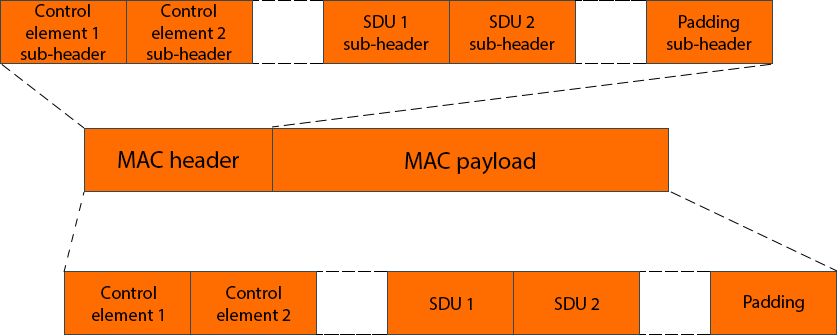
\includegraphics[width=0.8\textwidth]{images/mac_pdu.png}}
	\caption{Struktura pakietu PDU}
	\label{fig:mac_pdu}
\end{figure}

\begin{figure}
	\centerline{
\includegraphics[width=0.8\textwidth]{images/mac_pdu_subheader.png}}
	\caption{Struktura elementu nagłówka PDU}
	\label{fig:mac_pdu_subheader}
\end{figure}

\section{Symulacja podwarstwy MAC}

Dla podwarstwy MAC przedstawiono kanały logiczne i transportowe a także mechanizm multipleksacji oraz priorytetyzacji. Rys. \ref{fig:mac_simulation}.

\begin{figure}[ht]
	\centerline{\frame{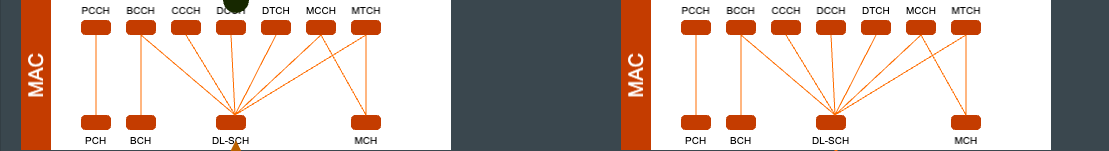
\includegraphics[width=0.9\textwidth]{images/mac_simulation.png}}}
	\caption{Symulacja podwarstwy MAC}
	\label{fig:mac_simulation}
\end{figure}


\chapter{Szczegóły implementacyjne symulacji}
\label{cha:symulacja}

\section{Wybór technologi}

Do wykonania symulacji zdecydowano się na wykorzystanie technologi przeglądarkowych. Obecnie, aplikacje działające w obrębie przeglądarki internetowej, są bardzo dynamicznie rozwijającym się obszarem inżynierii oprogramowania. Dzięki temu dostępna jest duża liczba narzędzi i bibliotek pozwalających na tworzenie aplikacji praktycznie dowolnego typu w tym właśnie symulacji oraz wizualizacji. Dodatkową zaletą aplikacji przeglądarkowych jest ich przenośność dzięki czemu możliwe jest ich uruchomienie na praktycznie każdym urządzeniu, które posiada zainstalowaną przeglądarkę internetową.
Poniżej opisano technologie na których przede wszystkim opiera się wykonana symulacja:

\subsection{Język programowania Typescript}

Jedynym językiem programowania wspieranym natywnie przez przeglądarki internetowe jest obecnie Javascript. Jednak dzięki odpowiednim narzędziom tzw. transpilerom jest możliwe pisanie kodu w innym języku a następnie przekształceniu go do języka Javascript.
W projekcie zdecydowano się na wykorzystanie języka Typescript. Jest to język stworzony przez firmę Microsoft i jest on transpilowany do języka Javascript. Posiada on składnię zbliżoną do języka Javascript dodatkowo jednak oferuje on przede wszystkim mechanizm statycznego typowania dzięki czemu możliwe jest wychwycenie błędów związanych z typami już na etapie kompilacji a nie jak w przypadku języków z dynamicznym typowaniem dopiero podczas działania aplikacji. W opini autora aplikacji pozwoliło to na łatwiejszą pracę z kodem, zwiększenie jego czytelności oraz zmniejszając liczbę potencjalnych błędów.

\subsection{Biblioteka renderująca Pixi.js oraz WebGL}

Wizualizacja zachowania się stosu protokołów oraz przepływu pakietów wymaga efektywnego wyświetlania na ekranie skomplikowanej hierarchi wielu obiektów. W tym celu wykorzystano bibliotekę Pixi.js oferującą interfejs pozwalający na tworzenie hierarchi obiektów, dokonywanie przekształceń geometrycznych i rysowanie podstawowych obiektów graficznych takich jak linie, elipsy, wielokąty. Biblioteka wykorzystuje niskopoziomowe API dostarczane przez przeglądarkę o nazwię WebGL. WebGL pozwala na efektywne renderowanie grafiki dwu oraz trójwymiarowej bezpośrednio w przeglądarce i na wykorzystanie możliwości oferowanych przez nowoczesne karty graficzne.

\subsection{Tween.js - animacje}

Większość animacji wykonano przy wykorzystaniu techniki nazywanej jako ``inbetweening`` zaimplementowanej w bibliotece Tween.js. Technika polega na wykorzystaniu funkcji interpolującej w celu wygenerowania płynnego przejścia pomiędzy początkowym i końcowym stanem obiektu. 
Na przykładzie animacji polegającej na przesunięciu obiektu z jednej pozycji na inną technika ta generuje wszystkie pośrednie pozycje obiektu mając podaną pozycję początkową oraz końcową. Dodatkowo na charakter animacji wpływa funkcja użyta do interpolacji. Użycie funkcji liniowej powoduje, że obiekt porusza się ruchem jednostajnym i zatrzymuje się natchmiast w miejscu co nie wygląda naturalnie. Natomiast użycie funkcji sinusoidalnej lub kwadratowej daje znacznie bardziej realistyczne wrażenie ponieważ obiekt stopniowo przyśpiesza a następnie zwalnia.

\section{Architektura aplikacji}

\begin{figure}[ht]
	\centerline{\frame{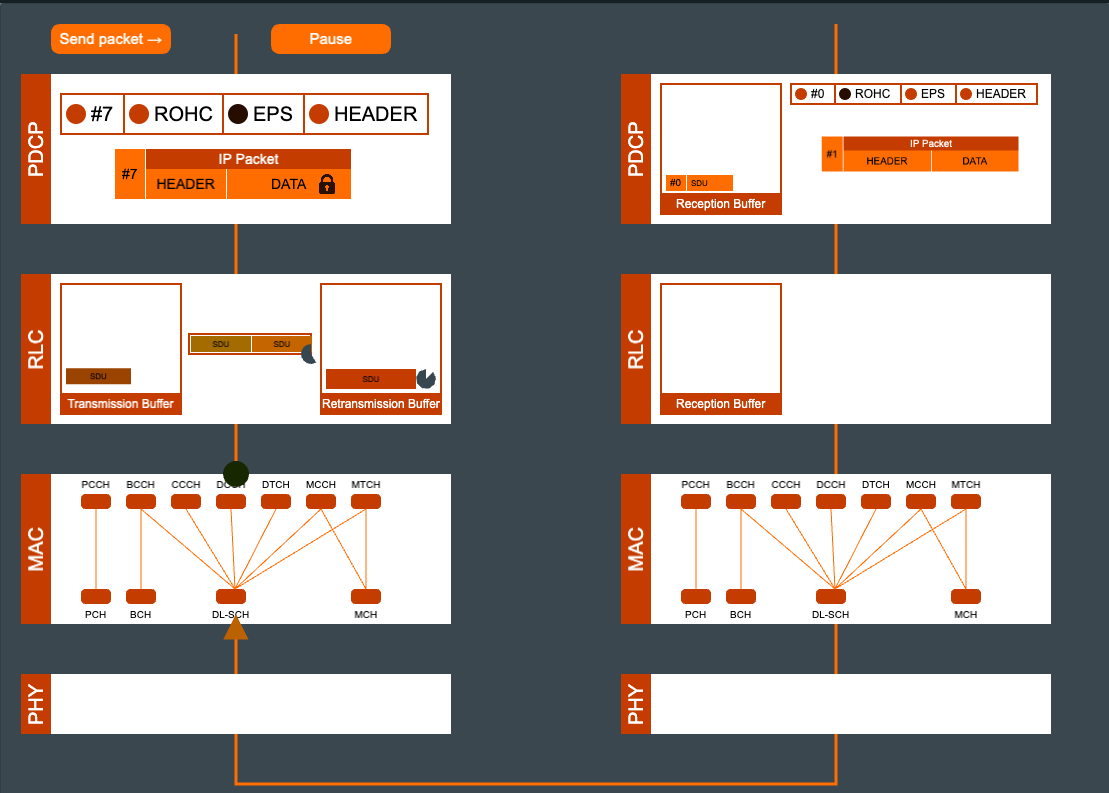
\includegraphics[width=0.8\textwidth]{images/simulation.png}}}
	\caption{Zrzut ekranu z wykonanej symulacji}
	\label{fig:simulation}
\end{figure}

Większość elementów widocznych na symulacji (Rys. \ref{fig:simulation}) została zaimplementowana jako osobne, niezależne obiekty. Każdy z obiektów zawiera logikę odpowiedzialną za jego wyświetlanie na ekranie jak i logikę odpowiedzialną za zamodelowanie odpowiadających mu mechanizmów związanych ze stosem protokołów LTE. Większość klas zaimplementowanych w ramach symulacji dziedziczy pośrednio lub bezpośrednio po klasie PIXI.Graphics dzięki czemu obiekty tej klasy mogą być renderowane, umieszczane w hierarchi obiektów a także mogą być na nich dokonywane transformacje geometryczne.

Poniżej opisano najbardziej kluczowe komponenty użyte w symulacji:

\subsection{Klasa Simulation}

Diagram UML dla klasy Simulation przedstawiono na Rys. \ref{fig:simulation_class}. Zawiera ona obiekty wszystkich symulowanych warstw, połączenia między nimi a także odpowiada za ich inicjalizację. Zawiera również obiekt klasy IPPacketGenerator odpowiadający za generowanie pakietów IP o losowej długości i inicjuje jego połączenie z przyciskiem ``Send packet``. Dzięki temu wciśnięcie przycisku powoduje wygenerowanie nowego pakietu IP i wysłanie go do pierwszej symulowanej podwarstwy tj. PDCP.

\begin{figure}[ht]
	\centerline{\frame{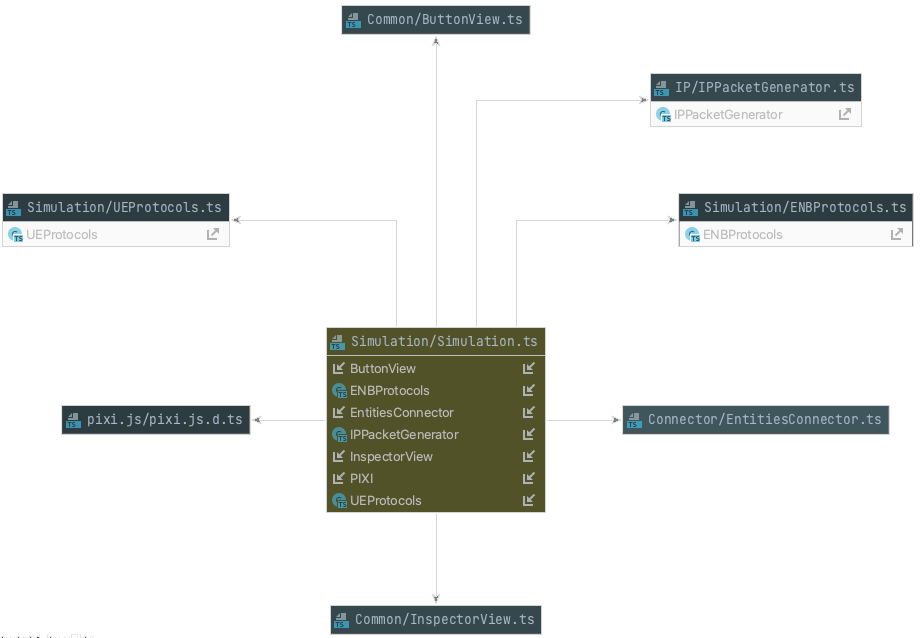
\includegraphics[width=0.8\textwidth]{images/simulation_class.png}}}
	\caption{Diagram UML dla klasy Simulation}
	\label{fig:simulation_class}
\end{figure}

\subsection{Klasa abstrakcyjna Connectable i interfejs DataUnit}

Najczęściej symulowanym zachowaniem w projekcie jest przesyłanie jednostek danych z jednego miejsca w drugie. Dlatego jednym z podstawowych komponentów, szeroko używanych w symulacji jest klasa abstrakcyjna Connectable. Posiada ona 2 kanały: A oraz B które umożliwiają przesyłanie w dwóch kierunkach obiektów implementujących interfejs DataUnit. Pozwala to na:

\begin{enumerate}
	\item wysyłanie jednostek danych do obiektu
	\item wysyłanie jednostek danych z obiektu do innych obiektów, które są podłączone do któregoś z kanałów danego obiektu
	\item łączenie obiektów razem ze sobą przy użyciu kanałów
	\item implementację dowolnej logiki reagowania na pojawienie się danych w kanale w klasach dziedziczących po klasie Connectable
\end{enumerate}

Domyślna reakcja obiektów dziedziczących po klasie Connectable na pojawienie się jednostki w kanale to przesłanie obiektu do drugiego kanału. Oznacza to, że obiekty wysłane do kanału A zostają odebrane a następnie opublikowane na kanale B. Natomiast obiekty wysłane do kanału B zostają opublikowane na kanale A. Dzieki temu domyślnie, obiekty dziedziczące po klasie Connectable, zachowuja się jak przewodniki. Takie zachowanie można zaobserwować np. w komponentach łączących warstwy pomiędzy sobą. Natomiast klasy implementujące poszczególne warstwy nadpisują domyślne zachowanie poprzez dodanie logiki odpowiadającej za przetwarzanie odebranych jednostek danych, buforowanie ich czy dodawanie nagłówków przed przesłaniem dalej.

\begin{figure}[ht]
	\centerline{\frame{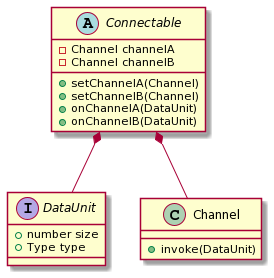
\includegraphics[width=0.5\textwidth]{images/connectable_class.png}}}
	\caption{Diagram UML dla klasy Connectable}
	\label{fig:connectable_class}
\end{figure}

\subsection{Klasa LayerView}

Implementuje części wspólne wszystkich podwarstw przedstawionych w symulacji. Tj. renderowanie nagłówka z nazwą podwarstwy oraz białego pola gdzie przedstawione są mechanizmy wchodzące w skład podwarstwy.

\subsection{Klasa BufferView}

W kilku miejscach symulacji można zauważyć wizualizację buforów przechowujących jednostki danych. Ich zachowanie polega na dodawaniu i usuwaniu jednostek danych a także układaniu ich w odpowiedniej kolejności. Ta logika została zaimplementowana przy użyciu klasy BufferView
\chapter{Podsumowanie}
\label{cha:podsumowanie}

Największym wyzwaniem podczas projektowania symulacji było znalezienie odpowiedniego balansu pomiędzy dokładnością przygotowanego modelu a ilością informacji prezentowanych na ekranie. Bardzo szczegółowy model wymaga przedstawienia tak wielu elementów, że symulacja staje się kompletnie nieczytelna. Natomiast model zbyt ogólny może nie posiadać elementów kluczowych do zrozumienia choćby podstawowych mechanizmów będących częścią stosu protokołów LTE.

Z wstępnie postawionych założeń udało się osiągnąć wykonanie symulacji kompletnego przepływu pakietu IP od urządzenia użytkownika do stacji bazowej. W tym przedstawiono udział wszystkich podwarstw warstwy 2. Szczególną uwagę poświęcono na implementacji mechanizmu ponownej transmisji i zapewnieniu dostarczenia pakietów w odpowiedniej kolejności na podwarstwie RLC.

Te elementy, które zostały zwizualizowane ogólnie, jak np. szyfrowanie na poziomie podwarstwy PDCP, posiadają dokładniejszy opis dostępny po kliknięciu myszą.

\section{Dalsze możliwości rozwoju}

Z powodu ograniczeń czasowych nie było możliwe zaimplementowanie wszystkich pomysłów autora symulacji. Poniżej wymieniono niektóre z nich:

\begin{enumerate}
	\item Dodanie większej liczby interaktywnych elementów. Obecna forma symulacji pozwala na wysłanie pakietu IP, przerwanie połączenia między urządzeniem użytkownika a stacją bazową a także pauzę symulacji. Do symulacji można dodać bardziej rozbudowane modyfikowanie parametrów połączenia, możliwość wysyłania pakietu IP zawierającego dane podane przez użytkownika oraz podgląd jednostek danych na każdym etapie jej przesyłania.
	\item Przedstawienie koncepcji nośników radiowych. W symulacji całkowicie pominięto kwestię istnienia nośników radiowych.
	\item Przedstawienie koncepcji płaszczyzny danych użytkownika (user plane) i płaszczyzny kontrolnej (control plane). Każda z przedstawionych podwarstw może działać w dwóch trybach w zależności od płaszczyzny danych. W obecnej wersji symulacji przedstawiono tylko płaszczyznę danych użytkownika
\end{enumerate}

\section{Wnioski}

Na podstawie wykonanego projektu cel pracy został osiągnięty. Osoba chcąca zapoznać się z tematem komunikacji pomiędzy urządzeniem użytkownika a stacją bazową w technologii LTE może skorzystać z wykonanej symulacji, aby lepiej zobaczyć jak poszczególne komponenty komunikują się ze sobą oraz jakie są odpowiedzialności. Autor ma nadzieję, że pozwoli to na zmniejszenia progu wejścia potrzebnego do zrozumienia podstaw a może i bardziej dogłębnego zrozumienia technologii jaką jest LTE.


\printbibliography

\end{document}

